\documentclass[12pt]{article}


\usepackage[utopia]{mathdesign}
\usepackage{graphicx}
\usepackage{amsmath}
%\interdisplaylinepenalty=2500
\usepackage{array}
\usepackage{amsthm}
\usepackage[colorlinks=true,pagebackref,linkcolor=magenta]{hyperref}
\usepackage{natbib}
\usepackage{enumerate}
\usepackage{bm}
\usepackage{bbm}
\usepackage{tikz}
\usetikzlibrary{shapes,arrows,external}


\newtheorem{theorem}{Theorem}[section]
\newtheorem{lemma}[theorem]{Lemma}
\newtheorem{corollary}[theorem]{Corollary}
\newtheorem{proposition}[theorem]{Proposition}
\newtheorem{assumption}{Assumption}
\theoremstyle{definition}
\newtheorem{definition}[theorem]{Definition}
\newtheorem{remark}[theorem]{Remark}

\renewcommand\arraystretch{1.2}
\newcommand{\argmax}{\operatornamewithlimits{argmax}}
\newcommand{\arginf}{\operatornamewithlimits{arginf}}
\newcommand{\argmin}{\operatornamewithlimits{argmin}}
\renewcommand{\tilde}{\widetilde}
\renewcommand{\hat}{\widehat}
\renewcommand{\Pr}{\mathbb{P}}
\renewcommand{\Re}{\mathbb{R}}

\title{SASD Pairs --- Permutation test}
\author{DLS}

\begin{document}
\maketitle

Two synapses are categorized into one of four type:
\begin{description}
  \item[SASD] Same axon and same dendrite ($n=35$).
  \item[DASD] Different axon and same dendrite ($n=166$).
  \item[SADD] Same axon and different dendrite ($n=8$).
  \item[DADD] Different axon and different dendrite ($n=1502$). 
\end{description}

We take all SASD pairs of dendrites and compare them to other SASD pairs to determine whether SASD pairs are more similar to each other than to other distinct SASD pairs.
We then permute which synapses are paired with which and recompute the statistics many times to compute a $p$-value for the 1-sided hypothesis test of whether the SASD pairs are more similar than the non-SASD pairs.
We also compare DADD pairs to pairs which share either an axon, a dendrite or both. 
Finally, we compare SASD to DASD pairs.
We do not compare SASD to SADD pairs due to the small sample size for SADD pairs. 

\textbf{Note:} If it is desired we can compare SASD pairs to the combination of DASD and SADD pairs and based on Figure~\ref{fig:density} it seems that the effect size would increase for most of the features. 

\section{Overview}
\begin{description}
\item[SASD vs. non-SASD pairs] We compared SASD pairs to non-SASD pairs for all 5 features. We conclude that SASD pairs are statistically significantly more similar for the $\log_{10}$ of spine volume feature $(p=3.4\times 10^{-4}, p_{\text{adjusted}} = 0.003$. The adjustment takes into account only the 5 tests performed here and uses the method of (Benjamini and Yekutieli (2001)). For the remaining features, the test did not yield statistical significance but each of the features were more similar for SASD pairs than non-SASD pairs. (See Table~\ref{tab:sasdVSrest}).
\item[non-DADD vs. DADD pairs] Here we compared synapse pairs that were on different dendrites and different synapes to pairs that shared either the same dendrite, the same axon or both. 
Again spine volume showed highly significan differences between these groups and the other features were all more similar for non-DADD pairs with various levels of significan.
We did not adjust for multiple comparisons. (See Table~\ref{tab:restVSdadd})
\item[SASD vs. DASD] The previous two analyses do not rule out the possibility that SASD pairs  are more similar mostly because they share the same dendrite so we compared SASD to DASD pairs. 
Here the sample sizes were smaller and so were the effect sizes. 
Spine volume again showed the strongest effect. (See Table~\ref{tab:sasdVSdasd}.)
\item[DASD vs. DADD] Here we tried to analyze the effect of just sharing the same dendrite (see Table~\ref{tab:dasdVSdadd}). Again, spine volume was highly significant and interesting \# Mitos also showed a significant effect.
\end{description}

Figure~\ref{fig:density} shows densities for each of the three ``continuous'' variables on both the raw- and log-scales. 
This gives an overall view of the differences between the different groups for each feature. It also illustrates that the main difference is for SASD pairs vs each of the other synapse-pair types. 
Spine volume shows the biggest difference between SASD, DASD and DADD pairs. 
Please note that there are only 8 SADD pairs and so though the density looks very different it is not statistically significant due to the small sample size.

\begin{figure}[tb]
  \begin{center}
    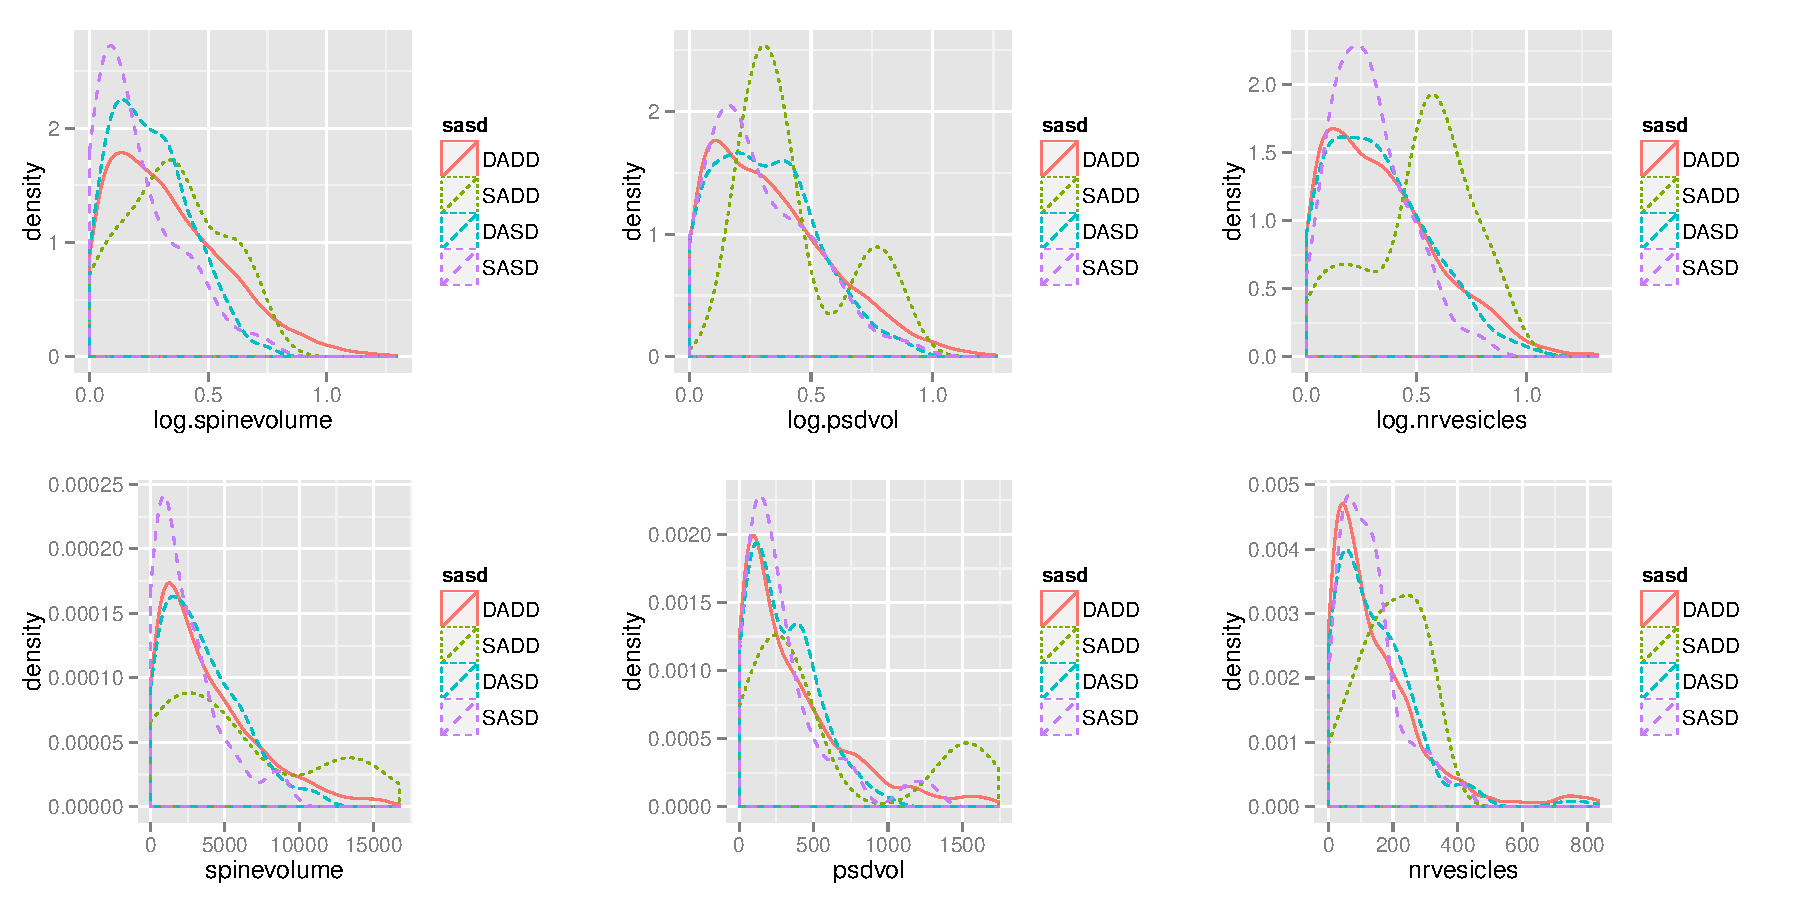
\includegraphics[width=\textwidth]{./Figures/sasdDensityPlots.pdf}
  \end{center}
  \caption{Densities for the differences for each of the three ``continuous'' variables on both the raw- and log-scales. }
  \label{fig:density}
\end{figure}

\begin{table}[tb]
  \label{tab:discreteCounts}
  \begin{center}
    \begin{tabular}{l|rcccc}
    \hline
                       &                & \textbf{DADD} & \textbf{SADD} & \textbf{DASD} & \textbf{SASD} \\ \hline
Same \# Mito.          & \textbf{True}  & 834 (55\%)          & 4   (50\%)          & 108   (65\%)        & 21 (60\%) \\
                       & \textbf{False} & 668           & 4             & 58            & 14 \\\hline
Same Spine App. Status & \textbf{True}  & 475  (46\%)         & 3  (37.5\%)         & 60  (36\%)         & 17 (48.5\%) \\
& \textbf{False}       & 1027           & 5             & 106           & 18 \\
    \hline
    \end{tabular}
  \end{center}
  \caption{Counts for how many discrete features are the same based on synapse pair type. }
\end{table}

\section{Comparing SASD to non-SASD synapse pairs}
  

\begin{table}[ht]\label{tab:sasdVSrest}
\caption{The name column indicates the synapse property of interest.
$\bar{X}_{SASD}$ is the mean difference for SASD pairs and $\bar{X}_{\neg SASD}$ is the mean difference for non-SASD pairs for the feature.
 The $p$-value indicates the percentage of permutations that had a difference $\bar{X}_D-\bar{X}_S$ that was larger than the the true difference. 
 The Adjusted column indicates the $p$-value after adjusting for multiple comparisons within just the 5 tests here. }
\centering
\textbf{Comparing SASD to non-SASD pairs}\\
\begin{tabular}{lrrrrr}
  \hline
Feature                          & $\bar{X}_{SASD}$ & $\bar{X}_{\neg SASD}$ & Difference & $\approx p$-value      & (Adjusted)\\
  \hline
$\log_{10}$ Spine Volume     & 0.2016           & 0.3269                & 0.1252    & $3.4\times 10^{-4}$  & 0.003  \\
$\log_{10}$ PSD Volume       & 0.2876           & 0.3379                & 0.05      & 0.11   & 0.322  \\
$\log_{10}$ \# Vesicles      & 0.2896           & 0.3476                & 0.058     & 0.08  & 0.322  \\
Spine Apparatus \%Diff. & 51\%             & 68\%                  & 16\%      & 0.014  & 0.084  \\
Number Mitos \%Diff.    & 40\%             & 43\%                  & 3.56\%    & 0.27  & 0.636  \\
   \hline
\end{tabular}
\end{table}

% Compare SASD to the Rest

% Comparing log.spinevolume
% Source: local data frame [2 x 2]

%    sasd mean(log.spinevolume)
% 1 FALSE             0.3268879
% 2  TRUE             0.2016551
% [1] -0.1252327
% [1] 0.00032
% Comparing log.psdvol
% Source: local data frame [2 x 2]

%    sasd mean(log.psdvol)
% 1 FALSE        0.3379041
% 2  TRUE        0.2875861
% [1] -0.05031796
% [1] 0.11093
% Comparing spineapp
% Source: local data frame [2 x 2]

%    sasd mean(spineapp)
% 1 FALSE      0.6789976
% 2  TRUE      0.5142857
% [1] -0.1647119
% [1] 0.01474
% Comparing nrmitos
% Source: local data frame [2 x 2]

%    sasd mean(nrmitos)
% 1 FALSE     0.4355609
% 2  TRUE     0.4000000
% [1] -0.03556086
% [1] 0.27793
% Comparing log.nrvesicles
% Source: local data frame [2 x 2]

%    sasd mean(log.nrvesicles)
% 1 FALSE            0.3476072
% 2  TRUE            0.2896035
% [1] -0.05800376
% [1] 0.08442



\begin{table}[tb]
  \caption{Comparison of synapse pairs which share either a dendrite, an axon or both, ($\neg$DADD, $n=209$) to DADD synapses ($n=1502$). 
  Here the $\neg$DADD are seen to be more similar on average than DADD pairs. 
  The spine volume is highly significan and the other features are all more similar for synapse pairs that share at least an axon or a dendrite. 
  Note that we did not adjust for multiple comparisons.}
  \label{tab:restVSdadd}
  \begin{center}
    \begin{tabular}{l|cccc}
    \hline

    \hline
Feature                  & $\bar{X}_{\neg DADD}$ & $\bar{X}_{DADD}$ & Difference & $\approx p$-value  \\
    \hline
$\log_{10}$ Spine Volume & 0.250                 & 0.334            & 0.084      & 0     \\
$\log_{10}$ PSD Volume   & 0.311                 & 0.340            & 0.028      & 0.052 \\
$\log_{10}$ \# Vesicles  & 0.328                 & 0.348            & 0.020      & 0.130 \\
Spine Apparatus \% Diff. & 61.7\%                & 68.3\%           & 6.6\%     & 0.023 \\
\# Mitos \% Different    & 36.3\%                & 44.4\%           & 8.1\%     & 0.010 \\
    \hline
    \end{tabular}
  \end{center}
\end{table}

% \begin{verbatim}


% Compare DADD to the rest

% Comparing log.spinevolume
% Source: local data frame [2 x 2]

%    sasd mean(log.spinevolume)
% 1 FALSE             0.3345960
% 2  TRUE             0.2505206
% [1] -0.08407539
% [1] 0
% Comparing log.psdvol
% Source: local data frame [2 x 2]

%    sasd mean(log.psdvol)
% 1 FALSE        0.3403889
% 2  TRUE        0.3116203
% [1] -0.02876861
% [1] 0.05289
% Comparing spineapp
% Source: local data frame [2 x 2]

%    sasd mean(spineapp)
% 1 FALSE      0.6837550
% 2  TRUE      0.6172249
% [1] -0.06653011
% [1] 0.02326
% Comparing nrmitos
% Source: local data frame [2 x 2]

%    sasd mean(nrmitos)
% 1 FALSE     0.4447403
% 2  TRUE     0.3636364
% [1] -0.08110398
% [1] 0.01078
% Comparing log.nrvesicles
% Source: local data frame [2 x 2]

%    sasd mean(log.nrvesicles)
% 1 FALSE            0.3489350
% 2  TRUE            0.3283516
% [1] -0.0205834
% [1] 0.1306

% Adjusted $p$-values via BY[1] 1 1 1 0 1



\begin{table}[tb]
  \caption{Comparison of SASD ($n=35$) synapse pairs to DASD ($n=166$) synapse pairs to test the effect of same axon among synapse pairs that have the same dendrite.
  Here we see that the effect sizes are smaller on the whole than in the other two comparisons. Again the spine volume difference seems to be the strongest.
  All but the \# Mitos feature are more similar for SASD pairs than for DASD pairs.
  Note that we did not adjust for multiple comparisons. }
  \label{tab:sasdVSdasd}
  \begin{center}
    \begin{tabular}{l|cccc}
    \hline

    \hline
Feature                  & $\bar{X}_{SASD}$ & $\bar{X}_{DASD}$ & Difference & $\approx p$-value  \\
    \hline
$\log_{10}$ Spine Volume & 0.201 & 0.256 & 0.054 & 0.037 \\
$\log_{10}$ PSD Volume   & 0.287 & 0.311 & 0.023 & 0.272 \\
$\log_{10}$ \# Vesicles  & 0.289 & 0.327 & 0.038 & 0.175 \\
Spine Apparatus \% Diff. & 51.4\% & 63.8\%& 12.4\% & 0.059 \\
\# Mitos \% Different    & 40.0\% & 34.9\% & -5.0\% & 0.648 \\
    \hline
    \end{tabular}
  \end{center}
\end{table}


% Compare SASD to DASDComparing log.spinevolume
% Source: local data frame [2 x 2]

%    sasd mean(log.spinevolume)
% 1 FALSE             0.2562536
% 2  TRUE             0.2016551
% [1] -0.05459845
% [1] 0.03762
% Comparing log.psdvol
% Source: local data frame [2 x 2]

%    sasd mean(log.psdvol)
% 1 FALSE        0.3112707
% 2  TRUE        0.2875861
% [1] -0.02368456
% [1] 0.27266
% Comparing spineapp
% Source: local data frame [2 x 2]

%    sasd mean(spineapp)
% 1 FALSE      0.6385542
% 2  TRUE      0.5142857
% [1] -0.1242685
% [1] 0.05989
% Comparing nrmitos
% Source: local data frame [2 x 2]

%    sasd mean(nrmitos)
% 1 FALSE     0.3493976
% 2  TRUE     0.4000000
% [1] 0.05060241
% [1] 0.64803
% Comparing log.nrvesicles
% Source: local data frame [2 x 2]

%    sasd mean(log.nrvesicles)
% 1 FALSE            0.3276086
% 2  TRUE            0.2896035
% [1] -0.0380051
% [1] 0.17516
% \begin{figure}[tb]
%   \begin{center}

%   \end{center}
%   \caption{Each figures illustrates a density estimate for the null distribution of the mean differences for the statistic $\bar{X}_{\neg SASD}-\bar{X}_{SASD}$ after performing 100,000 permutations of which synapses are SASD versus non-SASD. The vertical line indicates the  difference using the true SASD versus non-SASD pairs.}
%   \label{fig:meanDensity}
% \end{figure}
 

%  Comparing log.spinevolume
% Source: local data frame [2 x 2]



\begin{table}[tb]
  \caption{Comparison DASD ($n=166$) to DADD synapse pairs to test the effect of same dendrite.
  Here we again have a few highly significant results, notably for spine volume and interestingly \# Mitos. 
  Note that we did not adjust for multiple comparisons. }
  \label{tab:dasdVSdadd}
  \begin{center}
    \begin{tabular}{l|cccc}
    \hline

    \hline
Feature                  & $\bar{X}_{SASD}$ & $\bar{X}_{DASD}$ & Difference & $\approx p$-value  \\
    \hline
$\log_{10}$ Spine Volume & 0.256  & 0.334  & 0.078 & 1e-04 \\
$\log_{10}$ PSD Volume   & 0.311  & 0.340  & 0.029 & 0.072 \\
$\log_{10}$ \# Vesicles  & 0.327  & 0.348  & 0.021 & 0.147 \\
Spine Apparatus \% Diff. & 63.8\% & 68.3\% & 4.5\% & 0.1029 \\
\# Mitos \% Different    & 34.9\% & 44.4\% & 9.5\% & 0.0064 \\
    \hline
    \end{tabular}
  \end{center}
\end{table}

% Comparing log.spinevolume
% Source: local data frame [2 x 2]

%    sasd mean(log.spinevolume)
% 1 FALSE             0.3345960
% 2  TRUE             0.2562536
% [1] -0.07834243
% [1] 1e-04
% Comparing log.psdvol
% Source: local data frame [2 x 2]

%    sasd mean(log.psdvol)
% 1 FALSE        0.3403889
% 2  TRUE        0.3112707
% [1] -0.02911821
% [1] 0.0724
% Comparing spineapp
% Source: local data frame [2 x 2]

%    sasd mean(spineapp)
% 1 FALSE      0.6837550
% 2  TRUE      0.6385542
% [1] -0.04520078
% [1] 0.1029
% Comparing nrmitos
% Source: local data frame [2 x 2]

%    sasd mean(nrmitos)
% 1 FALSE     0.4447403
% 2  TRUE     0.3493976
% [1] -0.09534276
% [1] 0.0064
% Comparing log.nrvesicles
% Source: local data frame [2 x 2]

%    sasd mean(log.nrvesicles)
% 1 FALSE            0.3489350
% 2  TRUE            0.3276086
% [1] -0.02132642
% [1] 0.147

\begin{table}[tb]
  \caption{Comparison SASD ($n=35$) to SADD ($n=8$) synapse pairs to test the effect of same axon condition on same axon. Seems somewhat significant again. }
  \label{tab:dasdVSdadd}
  \begin{center}
    \begin{tabular}{l|cccc}
    \hline

    \hline
Feature                  & $\bar{X}_{SASD}$ & $\bar{X}_{SADD}$ & Difference & $\approx p$-value  \\
    \hline
log.spinevolume & 0.202 & 0.345 & 0.144 & 0.0364 \\ 
log.psdvol & 0.288 & 0.424 & 0.136 & 0.0585 \\ 
log.nrvesicles & 0.29 & 0.513 & 0.224 & 0.0039 \\ 
spineapp & 0.514 & 0.625 & 0.111 & 0.167 \\ 
nrmitos & 0.4 & 0.5 & 0.1 & 0.1796 \\ 
    \hline
    \end{tabular}
  \end{center}
\end{table}


\begin{table}[tb]
  \caption{Comparison SADD ($n=8$) to DADD ($n=1502$) synapse pairs to test the effect of same axon condition on same axon. Definitely not sigificant.  }
  \label{tab:dasdVSdadd}
  \begin{center}
    \begin{tabular}{l|cccc}
    \hline

    \hline
Feature                  & $\bar{X}_{SADD}$ & $\bar{X}_{DADD}$ & Difference & $\approx p$-value  \\
    \hline
log.spinevolume & 0.345 & 0.335 & -0.0108 & 0.5681 \\ 
log.psdvol & 0.424 & 0.34 & -0.0836 & 0.8173 \\ 
spineapp & 0.625 & 0.684 & 0.0588 & 0.2316 \\ 
nrmitos & 0.5 & 0.445 & -0.0553 & 0.494 \\ 
log.nrvesicles & 0.513 & 0.349 & -0.164 & 0.9608 \\ 
    \hline
    \end{tabular}
  \end{center}
\end{table}

\end{document}
